\documentclass[tikz,border=10pt]{standalone}
\usepackage{amsmath}
\usepackage{amssymb}
\definecolor{mantis}{RGB}{0, 105, 62}
\begin{document}
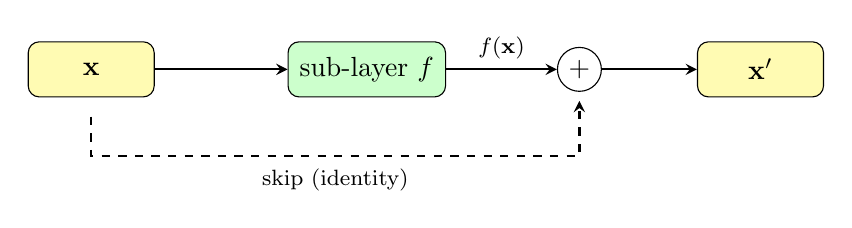
\begin{tikzpicture}[>=stealth]
    \node[draw, rounded corners, fill=yellow!30, minimum width=1.6cm, minimum height=0.7cm] (x) at (0,0) {$\mathbf{x}$};
    \node[draw, rounded corners, fill=green!20, minimum width=2cm, minimum height=0.7cm] (f) at (3.5,0) {sub-layer $f$};
    \node[draw, circle, fill=white, inner sep=2pt] (plus) at (6.2,0) {$+$};
    \node[draw, rounded corners, fill=yellow!30, minimum width=1.6cm, minimum height=0.7cm] (out) at (8.5,0) {$\mathbf{x}'$};
    \draw[->, thick] (x) -- (f);
    \draw[->, thick] (f) -- (plus) node[midway, above, font=\footnotesize] {$f(\mathbf{x})$};
    \draw[->, thick] (plus) -- (out);
    \draw[->, thick, dashed] (0,-0.6) -- (0,-1.1) -- (6.2,-1.1) -- (6.2,-0.4);
    \node[font=\footnotesize] at (3.1,-1.4) {skip (identity)};
\end{tikzpicture}
\end{document}
